\section{Proofs}
\label{app:proofs}

\subsection{Proposition~\ref{prop:filter}}

Fix $x$ and assume $\pi_{\mathrm{ref}}(\cdot\mid x)>0$, so the KL term is finite and every policy
on the path is strictly positive. The objective
$\sum_y \pi(y)r(x,y) - \beta\sum_y \pi(y)\log\frac{\pi(y)}{\pi_{\mathrm{ref}}(y)}$
over the simplex is strictly concave for $\beta>0$; setting the derivative of the Lagrangian to
zero gives $\pi^\star_\beta(y\mid x) = \pi_{\mathrm{ref}}(y\mid x)e^{r(x,y)/\beta}/Z_\beta(x)$ with
$Z_\beta(x)=\sum_{y'}\pi_{\mathrm{ref}}(y'\mid x)e^{r(x,y')/\beta}$. For $y,y'$ with
$r(x,y)=r(x,y')$ the normaliser and the exponential factor cancel in the ratio. Since $r\geq c$
we have $\Hset(x)\subseteq\Acc(x)$ and $r\equiv 1$ on $\Acc(x)$, so
\[
\frac{\pi^\star_\beta(\Hset(x)\mid x)}{\pi^\star_\beta(\Acc(x)\mid x)}
= \frac{e^{1/\beta}\pi_{\mathrm{ref}}(\Hset(x)\mid x)/Z_\beta(x)}{e^{1/\beta}\pi_{\mathrm{ref}}(\Acc(x)\mid x)/Z_\beta(x)}
= \frac{\pi_{\mathrm{ref}}(\Hset(x)\mid x)}{\pi_{\mathrm{ref}}(\Acc(x)\mid x)}
\]
for every $x$, hence $\rho$ and $\Lambda$ are unchanged; strict positivity makes $\rho$ finite,
and $\Lambda$ too whenever $\Hset(x)\neq\emptyset$. For a multiplicative update
$\pi_{t+1}(y\mid x)\propto\pi_t(y\mid x)e^{\eta f(r(x,y))}$ the same cancellation applies at
every step.

\paragraph{Excursion of the pooled statistic.} Write $a_x = \pi_{\mathrm{ref}}(\Acc(x)\mid x)$,
$\rho_x = \pi_{\mathrm{ref}}(\Hset(x)\mid x)/a_x$ and $s=e^{1/\beta}$. Then
$\pi^\star_\beta(\Acc(x)\mid x) = s\,a_x/(1-a_x+s\,a_x)$, and the pooled statistic is
$P(s) = \sum_x \rho_x w_x(s)/\sum_x w_x(s)$ with $w_x(s)=s a_x/(1-a_x+s a_x)$. At $s=1$ (no RL)
$P = \sum_x a_x\rho_x/\sum_x a_x$; as $s\to\infty$ every $w_x\to1$, provided $a_x>0$ at every
prompt, and $P \to \frac1N\sum_x \rho_x = \rho(\pi_{\mathrm{ref}})$; a prompt of zero accepted
mass never enters, and the limit would then be the average over the accepting prompts only.
The total excursion is therefore
\[
P(\infty)-P(1) \;=\; \frac1N\sum_x \rho_x \;-\; \frac{\sum_x a_x\rho_x}{\sum_x a_x}
\;=\; -\,\frac{\Cov_x(a_x,\rho_x)}{\mathbb{E}_x[a_x]},
\]
which is positive whenever pass rate and hack fraction are negatively correlated across prompts.
The pooled statistic therefore drifts upward under pure filtering, and its total excursion
vanishes exactly when $\Cov_x(a_x,\rho_x)=0$. Constant $\rho_x$ is sufficient for that but not
necessary: if the accepted mass $a_x$ is the same at every prompt then so is $w_x(s)$, and
$P(s)=\frac1N\sum_x\rho_x$ for every $s>0$ however much $\rho_x$ varies, as shown by
$a=(\tfrac12,\tfrac12)$ with $\rho=(0,1)$. It is not an estimator of $\rho$ and we do not call it
unbiased; it is a deterministic function of the filtering path that happens to converge to $\rho$
in the strong-RL limit.

\subsection{Lemma~\ref{lem:drift}}

$\nabla_\theta J = \frac1N\sum_{x'}\sum_{y'}\pth(y'\mid x')r(x',y')\nabla_\theta\log\pth(y'\mid x')
= \frac1N\sum_{x'}\mathbb{E}_{y'}[r(x',y')\nabla_\theta\log\pth(y'\mid x')]$.
Since $\mathbb{E}_{y'}[\nabla_\theta\log\pth(y'\mid x')]=0$, the expectation equals
$\Cov_{y'}(r,\nabla_\theta\log\pth)$, understood componentwise. For a fixed vector
$v=\nabla_\theta\log\pth(y\mid x)$, $\langle v,\Cov(r,g)\rangle = \mathbb{E}[r\langle
v,g\rangle]-\mathbb{E}[r]\mathbb{E}[\langle v,g\rangle]=\Cov(r,\langle v,g\rangle)$,
so the inner product passes inside. \qed

\subsection{Corollary~\ref{cor:tabular}}

With $\theta=(\theta_x)$ and $\pth(\cdot\mid x)$ a function of $\theta_x$ only,
$\nabla_{\theta_{x'}}\log\pth(y\mid x)=0$ for $x'\neq x$, so every off-diagonal kernel entry is a
sum of products with a zero factor. Moreover
$\nabla_{\theta_x}J=\frac1N\sum_y\pth(y\mid x)(r(x,y)-V(x))\nabla_{\theta_x}\log\pth(y\mid x)$
involves only $\theta_x$, so the flow restricted to block $x$ is autonomous and depends on the
verifier only through $r(x,\cdot)$. \qed

\paragraph{Rich-get-richer under vanilla policy gradient.} For a single prompt with free logits
$\theta_y$ and $J=\sum_y\pi_y r_y$, $\partial J/\partial\theta_z = \pi_z(r_z-J)$, so for two
responses with $r_1=r_2=1$,
$\frac{d}{dt}\log(\pi_1/\pi_2)=\dot\theta_1-\dot\theta_2=(\pi_1-\pi_2)(1-J)$. In the $N$-prompt
per-prompt-parameter setting of Corollary~\ref{cor:tabular} the objective carries a $1/N$ and
the baseline is the prompt's own pass rate,
$\partial J/\partial\theta_{x,z}=\frac1N\pth(z\mid x)(r(x,z)-V(x))$, so the rate quoted in
Section~\ref{sec:theory} is $\frac1N(\pi_1-\pi_2)(1-V(x))$; the two agree at $N=1$, where $J=V$.
The odds between equally rewarded responses are therefore \emph{not} preserved by vanilla policy
gradient, even with no parameter sharing; they move toward whichever response already has more
mass, at a rate that vanishes only as $V(x)\to1$. This is the prompt-local drift referred to in
Section~\ref{sec:theory}; it is independent of $u$ by Corollary~\ref{cor:tabular}.

\subsection{Proposition~\ref{prop:threshold}}

Two parts of the kernel drop out before Definition~\ref{def:coherent} is applied: any component of
$\Kk((x,h),(x',y'))$ that does not depend on $y'$ contributes zero covariance in \eqref{eq:drift},
and any component that does not depend on $h$ is common to the leak and to the correct answer and
cancels in the within-prompt log-odds. Substituting the definition, the covariance at $x'$ is
\[
\begin{aligned}
\Cov_{y'}[r(x',y'),\Kk((x,h),(x',y'))]
&= \kappa\Big(\pth(h\mid x')r(x',h) - \pth(h\mid x')V(x')\Big) \\
&= \kappa\,\pth(h\mid x')\big(r(x',h)-V(x')\big),
\end{aligned}
\]
using $\mathbb{E}_{y'}[r]=V(x')$, with $\kappa$ replaced by $\kappa_s$ in the $x'=x$ term. Since
$r(x',h)=\mathbf{1}[x'\in U]$, for $x\in U$,
\[
\begin{aligned}
\frac{d}{dt}\log\pth(h\mid x)
&=\frac{\kappa}{N}\Big[\sum_{x'\in U\setminus\{x\}}\!\!\pth(h\mid x')(1-V(x'))
-\sum_{x'\notin U}\pth(h\mid x')V(x')\Big] \\
&\quad + \frac{\kappa_s}{N}\pth(h\mid x)(1-V(x)).
\end{aligned}
\]
With $\pth(h\mid\cdot)\equiv p_h$ and $V\equiv\bar V$ the bracket is
$p_h[(m-1)(1-\bar V)-(N-m)\bar V] = p_h[N(u-\bar V)-(1-\bar V)]$, giving
$\kappa p_h(u-\bar V) + \frac{p_h(1-\bar V)}{N}(\kappa_s-\kappa)$. For $x\notin U$ the same
computation gives $\kappa p_h(u-\bar V) - \frac{p_h\bar V}{N}(\kappa_s-\kappa)$: the leading term
is unchanged and only the $1/N$ correction differs, its $1-\bar V$ becoming $-\bar V$. The
identical computation for $g_x$ with scales $(\kappa_g,\kappa_{s,g})$ and universality $u_g$
gives $\kappa_g p_g(u_g-\bar V) + \frac{p_g(1-\bar V)}{N}(\kappa_{s,g}-\kappa_g)$, so
subtracting leaves
\[
\kappa\,p_h(u-\bar V) \;-\; \kappa_g\,p_g(u_g-\bar V)
\;+\; \frac{1-\bar V}{N}\Big[(\kappa_s-\kappa)\,p_h - (\kappa_{s,g}-\kappa_g)\,p_g\Big],
\]
which is \eqref{eq:threshold} at $\kappa_g=0$, where the only mass on the correct answer that
survives is $p_g=\pth(g_x\mid x)$. \qed

\paragraph{Validity of the leading-order threshold.} The $1/N$ correction in
\eqref{eq:threshold} is $O(1/N)$ at fixed kernel scales, but it is small \emph{relative to the
leading term} only when $N\kappa/\kappa_s \gg 1$, which is a condition on the kernel and not on
$N$ alone. We measure $\kappa/\kappa_s$ as the mean cross-prompt gradient cosine for
the leak, and it is not constant: \CohHackHiFine{} at $u=1$ gives
$N\kappa/\kappa_s \approx \NThreshValidity{}$, but \CohHackLoFine{} at $u=\NuTwoLoU{}$ gives
$N\kappa/\kappa_s \approx 1.1$, at which point the correction is of the same order as the leading
term. The leading-order threshold is therefore an argument about the high-universality end only;
the suppression we observe at low $u$ is an empirical finding, not a prediction of
\eqref{eq:threshold}. Proposition~\ref{prop:threshold} also treats $\kappa$ as a constant while we
measure it growing roughly seventeenfold with $u$, so the observed growth of the cross-prompt drift
is jointly attributable to $\kappa(u)$ and to $(u-\bar V)$ and the proposition does not separate
them. Both are reasons we do not read a numerical boundary off the experiments.

\paragraph{Reading the threshold.} $\bar V$ is the policy's \emph{verifier} pass rate, observable
during training without any ground truth. A leak is amplified when it is accepted more often than
the policy currently passes. The statement is directional and first-order: it identifies the sign
of the leading-order drift and the quantity controlling it, not an exact boundary in a model whose
kernel is only approximately coherent.

\section{Environment, model and training details}
\label{app:details}

\paragraph{Task.} Prompts are all $(a,b)$ with $a,b\in\{2,\dots,9\}$ ($N=64$); the correct response
is the two-digit decimal string of $ab$ (all products lie in $[4,81]$). The response space is all
$100$ two-digit strings. Reducing the operand set to $\{2,\dots,5\}$ gives $N=16$ for the
prompt-set-size sweep, which uses three seeds and the learning-rate grid
$\{3\times10^{-4},10^{-3},3\times10^{-3}\}$ shared by both arms. The correct answers are not
perfectly prompt-specific ($2\times6$ and $3\times4$ both give $12$),
so they carry a universality of their own, $u_g=\NGoldU{}$. Under
Definition~\ref{def:coherent} what matters is measured coherence rather than string identity, and
we find the correct responses to be near-incoherent across prompts (\CohGold{}) while the leak is
not. $u_g$ is small and non-zero, and we report it rather than assume it away.

\paragraph{Leak assignment.} Leak strings are drawn without replacement from the $69$ two-digit
strings that are not the correct answer of any prompt, so a leak is never a correct answer
anywhere and every response is unambiguously classified. Prompts are partitioned into $N/m$
blocks; each block receives $k$ leak strings shared by all its prompts. The verifier's static
false-positive rate is exactly $k/99$ in every condition, independent of $m$.

Blocks are contiguous in the default configuration, and with prompts enumerated first-operand-major
a contiguous block of size $m\geq8$ is exactly a set of first operands, a property the transformer
can read off a single input token. That would confound universality with how simple the
prompt-to-leak map is to represent, so we run the whole sweep a second time with block membership
given by a random permutation of prompts and leak strings drawn independently per $(m,k,\text{seed})$
rather than nested across $m$. Both versions appear in Figures~\ref{fig:universality} and~\ref{fig:mechanism}.

\paragraph{What the base model does and does not control.} The SFT target puts identical hack mass
on every prompt in every condition, but the realised base model is a shared-weight transformer that
fits a universal leak map slightly better than an idiosyncratic one, so the measured base hack
fraction still varies by \NuTwoBaseRhoSpread{} across universality conditions. We therefore report
\emph{drifts} from each run's own base model, $\Delta\rho$ and $\Delta\Lambda$, which
Proposition~\ref{prop:filter} makes exactly zero under the filter baseline and which are immune to
that residual mismatch. Absolute $\rho$ is shown alongside the base curve so both are visible.

In the universality$\times$error-rate factorial an additional correction is needed. The uniform
component of the SFT target would otherwise place mass on each of the $k$ leak strings, so base
hack mass would grow with $k$ and the two factors would not be separable. For that experiment the
uniform component is spread only over responses that are neither the correct answer nor a leak,
which makes total base hack mass exactly $\varepsilon$ for every $k$. The measured base
\emph{fraction} still varies, mean $\rho = \NuThreeBaseRhoLoK{}$ with spread
\NuThreeBaseRhoSpreadK{} across runs, because diverting the uniform floor also changes the mass
on the correct answer; it is the mass, not the fraction, that the design holds fixed. This is the one place where the SFT target differs
between experiments, and it is the version the factorial requires.

\paragraph{Base model.} A decoder-only transformer with $2$ layers, model dimension $64$,
$4$ heads and a $10$-way output head over digits ($101{,}706$ parameters) is trained for $600$
Adam steps at $3\times10^{-3}$ on the exact target
$q(y\mid x)=(1-\varepsilon)[\lambda_x\mathbf{1}[y=g_x]+(1-\lambda_x)\mathrm{Unif}(\Yset)]+\varepsilon\,\mathrm{Unif}(\Hset(x))$
with $\varepsilon=0.03$. Competence levels $\lambda_x$ are an evenly spaced grid on $[0,0.9]$
assigned by a fixed permutation with a seed independent of the block structure, so difficulty and
universality are uncorrelated by construction. Because the loss is against an exact target rather
than samples, the resulting base distribution is matched across universality conditions without
any per-condition calibration.

\paragraph{Tabular policy.} Free parameters $w_1\in\mathbb{R}^{N\times10}$ and
$w_2\in\mathbb{R}^{N\times10\times10}$ with
$\pi(y\mid x)=\mathrm{softmax}(w_1[x])_{y_1}\cdot\mathrm{softmax}(w_2[x,y_1])_{y_2}$. This
factorisation is complete: $10$ free first-token logits plus $10\times10$ free second-token
logits reach every strictly positive distribution on the $100$ responses for each prompt, the
$9+10\cdot9=99$ free directions of the parameterisation matching the dimension of the simplex.
Given the base
transformer's exact log-probabilities we set
$w_1 = \log\sum_{y_2}\pi(y\mid x)$ and $w_2 = \log\pi(y\mid x) - w_1$, which reproduces the base
distribution to within $10^{-4}$ in max-norm (asserted at run time).

\paragraph{RL.} The default objective is the exact-expectation policy gradient with the exact
mean baseline,
$\nabla_\theta J = \frac1N\sum_x\sum_y\pth(y\mid x)\,[r(x,y)-V(x)]\,\nabla_\theta\log\pth(y\mid x)$,
implemented as a weighted cross-entropy with detached weights. This is the infinite-group limit of
RLOO and Dr.\ GRPO and removes sampling noise from the
comparison. The sampled-GRPO experiment uses group size $8$, group-standard-deviation
normalisation and one inner epoch. Optimiser Adam (default) or SGD, $400$ steps, learning-rate grid
$\{3\times10^{-4},10^{-3},3\times10^{-3},10^{-2},3\times10^{-2}\}$ for Adam and
$\{0.3,1,3\}$ for SGD, applied identically to both policy classes in the sweeps where a grid is
shared (Table~\ref{tab:protocol}; E3 and E5 use a fixed neural/tabular pair, E6 two). The reported operating point
is, for each policy class and cell, the smallest learning rate whose final verifier reward is
within $10^{-3}$ of the best, which is what a practitioner without ground truth would select
(strict argmax in E6).

\paragraph{The mask-only controls (E9, E9b).} One checkpoint per seed serves every universality
condition. Its supervised target is contaminated with a shared string $h$ and a per-prompt string
$s_x$ at every prompt, in identical proportion in all conditions, so the initial policy, the
probability on each leak string and the initial tangent kernel are bit-identical across the sweep;
we verify the base probability on $h$ agrees to six decimals. The verifier then accepts $h$ on the
$m$ prompts in $U$ and, in E9, $s_x$ on the rest, giving exactly $N$ accepted wrong pairs and a
static false-positive rate of exactly $1/(|\Yset|-1)$ in every condition. E9b accepts nothing wrong
outside $U$, so every accepted wrong string is $h$ and its base mass is identical across
conditions, at the cost of a static false-positive
rate equal to $u/99$ and therefore rising with $u$. Note also that only the \emph{per-prompt} mass
on the accepted string is held fixed in E9b: the aggregate accepted-wrong base mass, and with it
base $\rho$, still scale with $u$ because fewer prompts accept anything wrong at small $m$. Both
that and the rising rate bias E9b's slope downward, which is why the shared-versus-per-prompt
comparison is made within the same base rather than across conditions. The rising rate which if anything biases E9b's slope downward given that a
higher rate mildly reduces hacking in our factorial. $U$ is nested across $m$, so adjacent
conditions differ only by which prompts switched.

The residual gradient in E9 is that the accepted string's base mass rises from \MaskFprBaseLo{} to
\MaskFprBaseHi{}: a shared-parameter SFT represents one string demonstrated at every prompt better
than $N$ distinct ones. We tried to remove it by reweighting the two families in the supervised
target until their realised probabilities matched, iterating a damped fixed point. The mean gap
closes to $6\times10^{-4}$ but the per-prompt gap does not, staying near $6\times10^{-3}$ against
probabilities of about $1.2\times10^{-2}$: the shared network cannot represent an arbitrary
per-prompt split. Universality and representational ease are therefore not independently
manipulable in a shared-parameter model, since sharing is the common cause of both, which is why we
bracket the confound with two designs rather than eliminating it in one. E9's and E9b's per-prompt arms
responding to that residual gradient is what Corollary~\ref{cor:tabular} permits, since the
corollary rules out $u$-dependence generated by the dynamics, not $u$-dependence inherited at
initialisation.

\paragraph{Per-prompt weight copies (E10).} $N$ independent copies of the same transformer, each
initialised from the shared base checkpoint and trained on its own prompt alone with the same
objective and optimiser, on the three smallest learning rates of the shared arm's grid. Copy $x$
only ever evaluates prompt $x$, so the copies are independent and training them in one loop is
equivalent to training them separately. The matched shared-parameter arm it is compared against is
E1 restricted to the same four universality conditions and the same ten seeds, with slopes averaged
per seed, which is why its slope (\SharedSlopeMatched{}) differs slightly from the seven-condition
figure quoted in Section~\ref{sec:results} (\NuTwoNeuralSlope{}).

\paragraph{Full specification.} Prompts are serialised as the token sequence
$[\textsc{bos}, a, b, y_1]$ over a vocabulary of $12$ symbols ($10$ digits plus
\textsc{bos} and a padding symbol), with learned token and learned absolute positional
embeddings, a causal mask, pre-norm blocks, $4$ heads, feed-forward width $4d = 256$ with GELU,
final \texttt{LayerNorm}, and a $10$-way output head shared across the two response positions.
Embeddings are initialised $\mathcal{N}(0, 0.02^2)$ and the remaining parameters use PyTorch
defaults. The correct response for prompt $(a,b)$ is the decimal string of the \emph{product}
$a\times b$, zero-padded to two digits, so $2\times3$ has correct response \texttt{06}; all
products lie in $[4,81]$ and the response space is every two-digit string \texttt{00}--\texttt{99}.
Optimisation is full-batch over all $N$ prompts with no minibatching and no gradient clipping.
Adam uses $\beta_1=0.9$, $\beta_2=0.999$, $\varepsilon=10^{-8}$ and zero weight decay; SGD uses no
momentum. A run's seed simultaneously sets the transformer initialisation, the leak-string draw
and, in E4, the rollout sampling; the competence permutation is drawn from a separate fixed seed
so difficulty is never correlated with the leak structure.

The default objective is exact-expectation policy gradient,
$\nabla_\theta J = \frac1N\sum_x\sum_y \pth(y\mid x)[r(x,y)-V(x)]\nabla_\theta\log\pth(y\mid x)$,
with $V(x)=\sum_y\pth(y\mid x) r(x,y)$ the exact mean baseline. E4 replaces it with sampled GRPO:
$G=8$ responses are drawn per prompt at temperature $1$ from the full enumerated distribution,
advantages are $(r_i-\mathrm{mean})/(\mathrm{std}+10^{-4})$ within each group, groups whose reward
standard deviation is zero contribute zero advantage and hence no gradient, and one inner epoch is
taken per batch with no importance ratio, no clipping and no reference-KL term, so the estimator is
group-normalised REINFORCE rather than a ratio-clipped PPO objective. E5 adds
$-\beta\,\mathrm{KL}(\pth(\cdot\mid x)\Vert\pi_{\mathrm{ref}}(\cdot\mid x))$ computed exactly in
closed form against the frozen base, not estimated from samples.

\paragraph{Measurement.} $\rho$, $\Lambda$ and true accuracy are computed from the exact
enumerated distribution $\pth(\cdot\mid x)$ over all $100$ responses at all $N$ prompts, at every
logged step; they are not Monte-Carlo estimates, and the only stochasticity is over seeds
(transformer initialisation, leak-string draw, and rollout sampling in the GRPO condition). Two
probes are exceptions: the gradient decomposition and the coherence measurement average over a
fixed random subsample of $24$ and $12$ prompts respectively, for cost.

Per-prompt log-odds are clipped to $\pm20$ before averaging, so a prompt whose leak mass has
collapsed cannot dominate $\Lambda$. In the headline Adam sweep this binds on a median of
$1.6\%$ of prompts (worst case $18.8\%$). It binds far harder where the policy collapses
outright, up to $81\%$ under SGD at $u=1$, but neither the SGD nor the GRPO sweep contributes a
reported $\Lambda$, and on the sweeps that do the ordering of every reported series is unchanged
at clipping thresholds of $20$, $40$, $60$ and $200$. The final metric of every run is recomputed in float64 from stored per-prompt masses, so
the $10^{-8}$ floor used during online logging does not enter any reported number.

The two null-model checks in Section~\ref{sec:results} agree to the last bit by construction:
$400$ steps of mirror descent at $\eta=0.05$ reach exactly $\pi_0 e^{20 r}$, which is the
$\beta=0.05$ endpoint of the KL grid. They are one computation checked two ways, not two
independent checks.

\paragraph{Per-experiment protocol.} Seeds, learning-rate grids and the operating-point rule vary
between experiments; Table~\ref{tab:protocol} records what was actually run.

\begin{table}[h]
\centering\footnotesize
\begin{tabular}{llcc@{\hspace{4pt}}l}
\toprule
 & sweep & seeds & learning rates & notes \\
\midrule
E1 & universality, contiguous blocks & 10 & 5, shared by both arms & headline sweep \\
E2 & universality, permuted blocks   & 3 & 4, shared by both arms & base spread \NuSixBaseSpread{} \\
E3 & universality $\times$ error rate & 3 & 1 pair ($10^{-3}$ / $3\!\times\!10^{-2}$) & clean SFT floor \\
E4 & sampled GRPO                     & 10 & 3, shared by both arms & $G=\NGrpoG{}$, std normalisation \\
E5 & KL sweep                         & 3 & 1 pair ($10^{-3}$ / $3\!\times\!10^{-2}$) & 6 values of $\beta$ \\
E6 & verifier hardening               & 3 & 2 & strict argmax on verifier reward \\
E7 & prompt-set size $N\in\{16,64\}$   & 3 & 3, shared by both arms & tests $u$ versus $m$ \\
E8 & plain SGD                        & 10 & 3, shared by both arms & robustness \\
E9 & mask-only, constant error rate    & 10 & 5, shared by both arms & one frozen base per seed \\
E9b & mask-only, constant leak mass    & 5 & 5, shared by both arms & one frozen base per seed \\
E10 & per-prompt weight copies         & 10 & 3 & same architecture as the shared arm \\
\bottomrule
\end{tabular}
\caption{What was run in each experiment. Where a grid is shared by both arms the operating point
is the smallest learning rate within $10^{-3}$ of the best verifier reward, chosen independently
for each arm.}
\label{tab:protocol}
\end{table}

\section{Additional results}
\label{app:extra}

\begin{figure}[htbp]
\centering
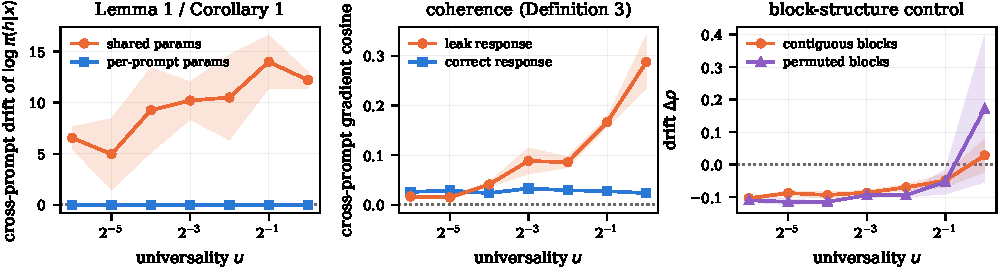
\includegraphics[width=\linewidth]{../figures/fig3_mechanism.pdf}
\caption{Mechanism. Left: the cross-prompt component of the exact drift of $\log\pth(h\mid x)$ at
the base model (Lemma~\ref{lem:drift}), identically zero for per-prompt parameters as
Corollary~\ref{cor:tabular} requires. Centre: mean pairwise cosine between per-prompt gradients,
the coherence of Definition~\ref{def:coherent}, measured rather than assumed. Right: contiguous
versus randomised block membership.}
\label{fig:mechanism}
\end{figure}

\begin{figure}[htbp]
\centering
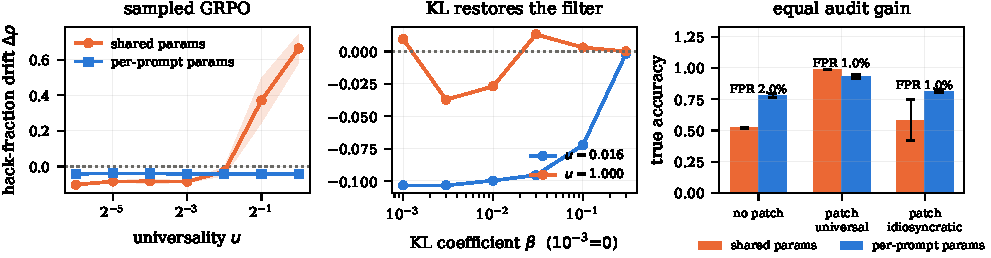
\includegraphics[width=\linewidth]{../figures/fig4_practice.pdf}
\caption{Practice. Left: sampled GRPO reproduces the pattern. Centre: a KL penalty pulls the policy
back toward the filter baseline; the low-$u$ side is resolved, the $u=1$ side is within noise. Right: two verifier patches that improve the
measured false-positive rate identically buy very different true accuracy.}
\label{fig:practice}
\end{figure}

\paragraph{Verifier hardening (E6).}

We give a verifier two leak families, one universal string plus one idiosyncratic string per
prompt, and compare two patches that remove exactly the same number of accepted wrong
(prompt, response) pairs and so improve any static audit identically. Removing the universal leak
leaves the policy at \NuFiveCAccU{} true accuracy; removing every idiosyncratic leak instead leaves
it at \NuFiveCAccI{}, a gap of $\NuFiveCGap{}\pm\NuFiveCGapSem{}$ points (\NuFiveCNSeeds{} seeds)
from patches an audit rates as equally valuable (unpatched: \NuFiveCAccNone{}). The per-prompt
policy, which by Corollary~\ref{cor:tabular} cannot respond to universality at all, shows a gap of
only \NuFiveCGapTab{} points between the same two verifiers. That residue is what the base model
already carried, since the SFT stage is itself shared-parameter (base hack fractions
\NuFiveCBaseU{} and \NuFiveCBaseI{}). The remaining \NuFiveCGapRL{} points are produced by RL.


\begin{figure}[htbp]
\centering
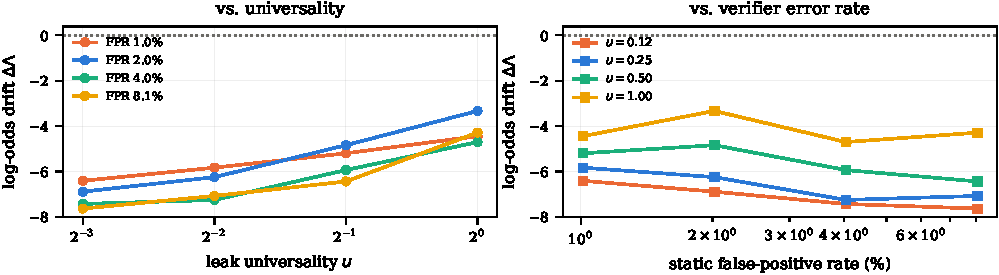
\includegraphics[width=\linewidth]{../figures/fig2_factorial.pdf}
\caption{In this environment universality moves the drift and the verifier's error rate does not.
Left: log-odds
drift against universality, one line per false-positive rate. Right: the same data against the
static false-positive rate, one line per universality, common $y$-scale. Varying accepted wrong
responses per prompt from \NuThreeKRange{} moves the false-positive rate over \NuThreeFprRange{}
and mildly \emph{reduces} hacking; universality moves the drift monotonically and much further.}
\label{fig:factorial}
\end{figure}

\paragraph{Prompt-set size (E7).} At fixed $u$ the analysis predicts no dependence on the number of prompts. Repeating the sweep at
$N=\NuFourNSmall{}$ and $N=\NuFourNBig{}$ is consistent with that: at $u=1$ the two agree
($\NuFourUOneSmall{}\pm\NuFourUOneSmallSem{}$ versus $\NuFourUOneBig{}\pm\NuFourUOneBigSem{}$),
whereas at the same block size $m=\NuFourSameM{}$ they sit at $\NuFourSameMBig{}$ against
$\NuFourUOneSmall{}$, a gap the three seeds do not resolve. Across the \NuFourNShared{} matched
values of $u$ the largest gap is \NuFourMatchedGap{}.

Figure~\ref{fig:appendix} collects the four robustness views that do not fit in the main text:
the universality effect across the whole Adam learning-rate grid rather than at the single
reward-selected operating point, hack-fraction trajectories at the two extreme universality
conditions for both policy classes, the sweep repeated at two prompt-set sizes, and the sweep
under plain SGD.

\begin{figure}[htbp]
\centering
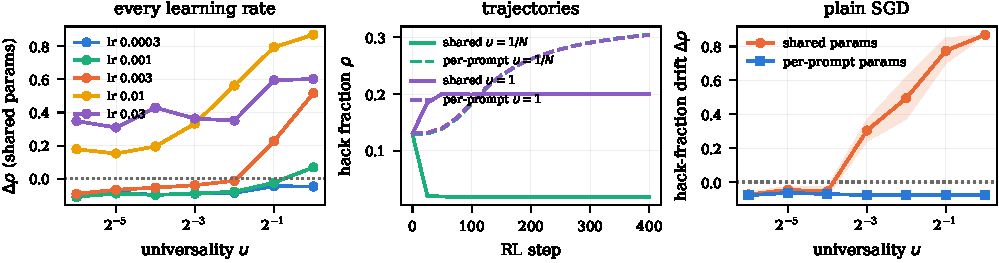
\includegraphics[width=\linewidth]{../figures/fig5_appendix.pdf}
\caption{Top left: the universality effect across the whole Adam learning-rate grid, rather than
at the reward-selected operating point; the ramp runs light (smallest step) to dark. Top right:
hack-fraction trajectories for the extreme universality conditions, both policy classes. Bottom
left: the sweep repeated at two prompt-set sizes, plotted against $u$. Bottom right: the same
universality sweep under plain SGD.}
\label{fig:appendix}
\end{figure}

\section{Reproducibility}

All code, raw result files and figure scripts are included with the submission. A single machine
with two CPU cores reproduces every experiment in the paper; no GPU is used. \texttt{src/env.py}
defines the task and verifier, \texttt{src/policies.py} the two policy classes,
\texttt{src/rlvr.py} the objectives and exact measurement, \texttt{src/theory.py} the numerical
verification of Proposition~\ref{prop:filter} and Lemma~\ref{lem:drift}, and
\texttt{src/exp*.py} the experiments. Seeds $0$--$4$ of E1 were produced by an earlier revision whose configuration records carry
fewer fields. Re-running a cell from that half under the current revision reproduces it to
$10^{-8}$ and the stored base models are bit-identical, so the halves are pooled. One cell of E1
(the $m=1$ condition) was run beyond the reported seed budget while a larger budget was being
attempted; \texttt{src/figures.py} caps every E1, E4, E8, E9, E9b and E10 load at its reported seed budget
and drops any seed not present at every universality condition, so the
reported design is balanced at ten seeds for every universality condition rather than giving a
few conditions more seeds than the rest. \texttt{src/figures.py} regenerates every figure and the
macro file holding every measured number quoted in the text; the hand-entered constants are the step count, the
contamination rate and the GRPO group size, which are settings rather than results, together with a
small number of measured figures quoted in the text rather than through a macro: the clipping
rates, $N\kappa/\kappa_s$, the seventeenfold growth of $\kappa$ and its peak at $u=0.5$, and the
leave-one-seed-out drift of $-0.017$, all recomputed from the shipped result files, and the three
probability gaps from the E9 reweighting attempt above, which come from a diagnostic run whose
output is not shipped.
